\documentclass[11pt]{article}
\usepackage[margin=1in]{geometry}
\usepackage{amsmath,amssymb,amsthm,mathtools}
\usepackage{graphicx}
\usepackage{microtype}
\usepackage[hidelinks]{hyperref}

\newtheorem{theorem}{Theorem}
\newtheorem{remark}{Remark}
\newcommand{\R}{\mathbb R}

\title{Injective Gradients Do Not Characterize Convexity\\
\large A counterexample to Conjecture 1 of arXiv:2106.04116}
\author{Autonomous proof candidate for human review}
\date{11 August 2026}

\begin{document}
\maketitle

\begin{center}
\fbox{\parbox{0.91\textwidth}{\textbf{Status.}
Candidate full counterexample, likely valid.  On $X=\R$, the globally
$1$-Lipschitz function
\[
 F(x)=-\sqrt{1+x^2}
\]
is strictly concave, but it satisfies every subgradient-intersection identity
required by Conjecture 1.}}
\end{center}

\section{The conjecture}

The source uses $\nabla F(x)$ for the Clarke subdifferential of a locally
Lipschitz function.  Its Conjecture 1 asserts that a Lipschitz function
$F:X\to\R$ is convex if and only if
\begin{equation}\label{eq:condition}
 \nabla F(x)\cap\nabla F(y)
 =\nabla F(tx+(1-t)y)
\end{equation}
whenever $0\leq t\leq1$ and
$\nabla F(x)\cap\nabla F(y)\ne\varnothing$.

\begin{figure}[ht]
 \centering
 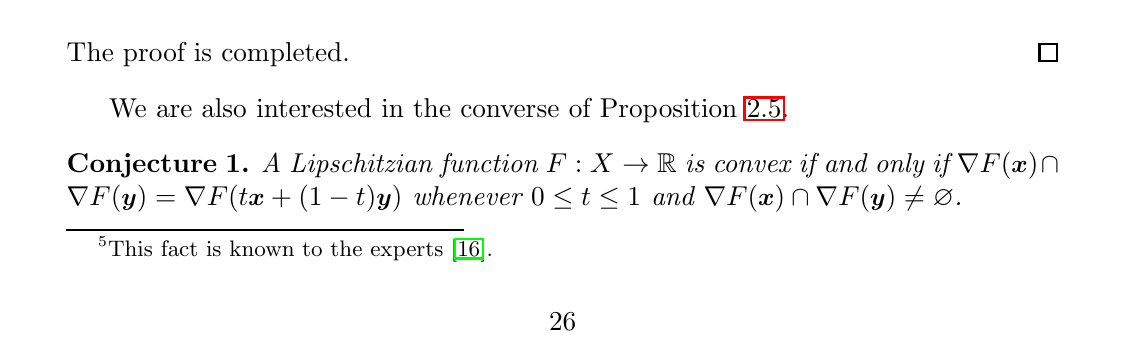
\includegraphics[width=\textwidth]{figures/problem_crop.png}
 \caption{Conjecture 1 in the source, PDF page 26.}
\end{figure}

The implication from convexity is the source's preceding proposition.  The
converse fails because the hypothesis says nothing about pairs of points whose
subdifferentials are disjoint.

\section{Counterexample}

\begin{theorem}\label{thm:counterexample}
The function $F:\R\to\R$ given by
\[
 F(x)=-\sqrt{1+x^2}
\]
is globally Lipschitz and nonconvex, yet satisfies \eqref{eq:condition} for
every $x,y\in\R$ and every $t\in[0,1]$ for which the conjecture requires it.
\end{theorem}

\begin{proof}
The function is continuously differentiable, with
\begin{equation}\label{eq:derivative}
 F'(x)=-\frac{x}{\sqrt{1+x^2}}.
\end{equation}
Since $|F'(x)|<1$, the mean value theorem shows that $F$ is globally
$1$-Lipschitz.  It is not convex: midpoint convexity at $-1$ and $1$ would
require
\[
 F(0)\leq\frac{F(-1)+F(1)}2,
\]
but this reads $-1\leq-\sqrt2$, which is false.  (Equivalently,
$F''(x)=-(1+x^2)^{-3/2}<0$.)

For a $C^1$ function, the Clarke subdifferential is the singleton containing
the ordinary derivative.  Hence
\[
 \nabla F(x)=\left\{-\frac{x}{\sqrt{1+x^2}}\right\}.
\]
The scalar function on the right is strictly decreasing, because its
derivative is $-(1+x^2)^{-3/2}<0$, and is therefore injective.  Consequently
\[
 \nabla F(x)\cap\nabla F(y)\ne\varnothing
 \quad\Longrightarrow\quad x=y.
\]
For the only pairs to which the conjectured condition applies, we thus have
$tx+(1-t)y=x=y$ for every $t\in[0,1]$, and
\[
 \nabla F(x)\cap\nabla F(y)
 =\nabla F(x)
 =\nabla F(tx+(1-t)y).
\]
This verifies the entire hypothesis, including both endpoints $t=0,1$, while
$F$ remains nonconvex.
\end{proof}

\section{Why the converse cannot work}

The counterexample is not tied to the particular square-root formula.  If a
smooth Lipschitz function on $\R$ has an injective derivative, then distinct
points have disjoint Clarke subdifferentials.  Condition
\eqref{eq:condition} is therefore vacuous off the diagonal and automatic on
the diagonal.  A bounded strictly decreasing derivative produces a concave
example; a bounded strictly increasing derivative produces a convex one.
The intersection identity by itself cannot distinguish them.

Thus any repaired converse needs a non-vacuity or monotonicity hypothesis
linking subgradients at distinct points.  The usual monotonicity condition
\[
 (p-q)(x-y)\geq0
 \qquad(p\in\nabla F(x),\ q\in\nabla F(y))
\]
does distinguish convex subdifferentials, but it is absent from Conjecture 1.

\section{Verification and novelty scope}

The example is one-dimensional, smooth, and globally Lipschitz, so it meets
the conjecture under either the global or local reading of ``Lipschitzian.''
It uses exactly the Clarke-subgradient convention stated in the source.  A
bounded search of the run indexes, exact conjecture wording, and the three
works indexed as citing the source located no prior discussion of this
counterexample.  Priority is not asserted.

The separate higher-dimensional Cheeger conjecture later in the same paper
is not addressed by this packet.

\begin{thebibliography}{9}
\bibitem{JS}
J.~Jost and D.~Zhang,
\emph{Discrete-to-continuous extensions: piecewise multilinear extension,
min-max theory and spectral theory},
arXiv:2106.04116.
\end{thebibliography}

\end{document}
